\documentclass[11pt]{beamer}
\usepackage{helvet} %font
\beamertemplatenavigationsymbolsempty
\usetheme{JuanLesPins}
\usefonttheme{structurebold}

\usepackage[french]{babel}
\usepackage[utf8]{inputenc}
\usepackage[T1]{fontenc}
\usepackage{amssymb,amsmath}
\usepackage{tikz}
\usepackage{geometry}
\usepackage{xcolor,colortbl}
\usetikzlibrary{arrows,positioning}
\usepackage{listings}

\AtBeginSubsection[]
{
   \begin{frame}
	\small \tableofcontents[currentsection]
   \end{frame}
}

\newenvironment{slide}[1]{%
\begin{frame}[environment=slide]
\frametitle{#1}
}{%
\end{frame}
}
\setbeamercolor{structure}{fg=red}
\setbeamercolor{frametitle}{bg=black,fg=white}
\definecolor{gris}{gray}{0.6}
\definecolor{grisclair}{gray}{0.9}

\newtheorem{exercice}{Exercice}

\title{Machine Learning - Tests}
\author{Nicolas Bourgeois}
\date{}

\newcommand{\Python}[1]{
	{\small	\lstinputlisting[language=Python]{./#1.py}}
}
\newenvironment{pyenvsmall}
	{ \ttfamily \tiny }
	{\par  }

\newcommand{\Pythonsmall}[1]{
	{\scriptsize \lstinputlisting[language=Python]{./#1.py}}
}
\newcommand{\elimine}[1]{{\textcolor{lightgray}{#1}}}


\begin{document}

\begin{frame}
\maketitle
\end{frame}
\section{Rappels}

\begin{slide}{Rappel des Hypothèses}
Observations :\\

\begin{itemize}

\item Variable empirique cible $\tilde{Y}$
\item Variables empiriques explicatives $\tilde{X}$

\end{itemize}

\pause

Hypothèses :\\

\begin{itemize}

\item $\tilde{X}$ est un ensemble d'observations lié à un processus aléatoire $X$
\item $\tilde{Y}$ est un ensemble d'observations lié à un processus aléatoire $Y$
\item il existe une relation $Y = f(X)$

\end{itemize}

\pause

Objectifs :\\

\begin{itemize}
\item Produire une fonction $\tilde{f}$ à partir de $\tilde{X}$ et $\tilde{Y}$
\item Telle que $\tilde{f}$ soit une approximation fiable de $f$
\item On pourra ainsi prédire $\tilde{Y}' = \tilde{f}(\tilde{X}')$ sur un nouvel échantillon 
\end{itemize}

\end{slide}


\begin{slide}{Erreur du modèle}

La bonne mesure serait de minimiser :

$$D(\tilde{f}) = \mathbb{E}(d(\tilde{f}(x),y))$$

Mais comme on ne connaît pas la loi de $(X,Y)$ c'est impossible.

\end{slide}


\begin{slide}{Erreur moyenne empirique}

On dispose d'un échantillon de test $\tau = (X_j,Y_j)_{j\leq n}$.\\

Minimiser :
$$\tilde{D}(\tilde{f},\tau) = \frac{1}{n}\sum_{j \leq m} d(\tilde{f}(x_j),y_j)$$

\pause

Ne pas confondre cette somme sur les données avec la somme sur les variables !\\
Ne pas confondre cette moyenne empirique avec la moyenne 
\end{slide}

\begin{slide}{Convergence}

D'après la loi des grands nombres, si les observations de test sont indépendantes, la moyenne empirique converge vers l'erreur du modèle.
\end{slide}

\begin{slide}{Pertinence du test}
On cherche à évaluer la probabilité que l'écart entre les deux mesures soit faible.

$$P\left(\tilde{D}(\tilde{f},\tau)-D(\tilde{f}) > \epsilon \right) < 1 - \rho$$

\end{slide}


\section{Tests Statistiques}

\begin{slide}{Test de Student monovarié}
On dispose d'une série d'observations $\tilde{X}$.\\
\pause
\vspace{0.2cm}On suppose que $\tilde{X}$ procède d'une loi inconnue $X \sim \mathcal{N}(\mu,\sigma^2)$.\\
\pause
\vspace{0.2cm}On veut évaluer l'espérance de cette loi $\mu$. 

\end{slide}

\begin{slide}{Test de Student monovarié}
On calcule la moyenne empirique sur un échantillon de taille n:
$$\bar{x} = \frac{1}{n}\sum_{x_i \in \tilde{X}} x_i.$$
\pause
Et l'écart-type empirique :
$$s = \sqrt{\frac{1}{n-1}\sum_{x_i \in \tilde{X}}(x_i-\bar{x})^2}$$

\end{slide}

\begin{slide}{Test de Student monovarié}
Hypothèse nulle : $\mu = \mu_0$ pour une certaine constante $\mu_0$.\\
\pause
\vspace{0.2cm}Conséquence : $\bar{x}\sim \mathcal{N}(\mu_0,\sigma/\sqrt{n})$.\\
\pause
\vspace{0.2cm}Donc la variable 
$$z=\sqrt{n}\frac{\bar{x}-\mu_0}{s}$$
suit une loi de Student à $n-1$ DL.

\end{slide}

\begin{slide}{Test de Student monovarié}
Méthode : on compare les observations de $z$ avec les valeurs attendues d'une loi de Student à $n-1$ DL.\\
\pause
\vspace{0.2cm} Si l'écart est trop important, on rejette l'hypothèse faite.
\end{slide}

\begin{slide}{Test de Student monovarié}
\begin{exercice}
Prélevez un échantillon de 30 valeurs se longueur de pétales sur les données iris. Calculez leur moyenne $m$, et testez l'hypothèse que les longueurs de pétales sont distribuées selon une loi normale de moyenne $m$.
\end{exercice}
\begin{exercice}
Générez un ensemble de 1000 valeurs suivant une loi normale centrée réduite. Testez l'hypothèse que ses valeurs sont distribuées selon une loi normale de moyenne $0$.
\end{exercice}
\end{slide}

\begin{slide}{Test de Student monovarié}

\Python{ex901}
\end{slide}


\begin{slide}{Test du $\chi^2$}
On dispose de deux séries d'observations $\tilde{X},\tilde{Y}$.\\
\pause
\vspace{0.2cm}On suppose que $\tilde{X},\tilde{Y}$ procèdent de lois inconnues $X,Y$.\\
\pause
\vspace{0.2cm}On veut déterminer si ces lois sont indépendantes ou corrélées. 

\end{slide}


\begin{slide}{Test du $\chi^2$}
On calcule les effectifs croisés espérés :
$$E_{i,j} = \frac{1}{n}\sum \sharp\{X=i\}\sharp\{Y=j\}$$
\pause
Les effectifs croisés observés :
$$O_{i,j} =  \sharp\{X=i \& Y=j\}$$
\pause
Et l'écart relatif entre les deux :
$$ T = \sum_{i,j}\frac{(O_{i,j}-E_{i,j})^2}{E_{i,j}}$$
\end{slide}


\begin{slide}{Test du $\chi^2$}
Hypothèse nulle : $X,Y$ sont indépendantes.\\
\pause
\vspace{0.2cm}Conséquence : $T$ suit une loi du $\chi^2$ à $(I-1,J-1)$ DL.

\end{slide}



\begin{slide}{Test du $chi^2$}
Méthode : on compare les observations de $T$ avec les valeurs attendues d'une loi du $\chi^2$ à $(I-1,J-1)$ DL.\\
\pause
\vspace{0.2cm} Si l'écart est trop important, on rejette l'hypothèse faite.
\end{slide}

\begin{slide}{Test du $\chi^2$}
\begin{exercice}
Construisez une table de contingence entre le genre et la classe sur les données du titanic. Testez l'hypothèse que la classe et le genre sont indépendants.
\end{exercice}
\begin{exercice}
Générez deux variables aléatoires indépendantes à deux modalités chacune. Construisez leur table de contingence et testez leur indépendance.
\end{exercice}
\end{slide}

\begin{slide}{Test du $\chi^2$}

\Pythonsmall{ex902}
\end{slide}


\section{Compromis Biais-Variance}

\begin{slide}{Biais-Variance}
2 parmi les grandes sources d'erreurs dans l'apprentissage :\\
\pause
\vspace{0.2cm}Le biais correspond au sous-apprentissage (modèle trop simple, trop peu de données)\\
\pause
\vspace{0.2cm}La variance correspond au surapprentissage (modèle apprend aussi le bruit)
\end{slide}



\begin{slide}{Biais-Variance}
Supposons une distribution bruitée $Y = f(X)+\epsilon$ avec $\epsilon$ de moyenne 0 et de variance $\sigma^2$.\\
\pause
$$E [(Y-{\tilde{f}}(X))^{2}] = E [(f(X)-{\tilde{f}}(X))]^{2} + E [({\tilde{f}}(X)-E[{\tilde{f}}(X)])^{2}] +\sigma^2$$
\end{slide}

\begin{slide}{Biais-Variance}
\begin{exercice}
Générez un vecteur X quelconque et un vecteur Y=3X+e où e est un bruit gaussien centré de variance s. Testez les variations du score d'une régression linéaire entre X et Y en fonction de s.
\end{exercice}
\end{slide}

\begin{slide}{Biais-Variance}
\Python{ex903}
\end{slide}

\section{Score}

\begin{slide}{Cross Validation}
On veut diviser efficacement nos données entre échantillons d'apprentissage et de test.\\

\vspace{0.2cm} La taille et la nature de ces divisions peuvent varier selon le classifieur employés, et scikit-learn en fournit en conséquence.

\end{slide}

\begin{slide}{Paramétrisation}
La cross validation peut être utilisée pour optimiser les paramètres d'un algorithme, soit entre eux, soit contre la complexité (ex. degré d'un kernel polynomial)
\end{slide}

\begin{slide}{Exercice}
\begin{exercice}
Calculez et affichez le cross-validation score d'un svm linéaire sur le jeu de données \texttt{digits}~en fonction de différentes valeurs du paramètre de régularisation C.
\end{exercice}
\begin{exercice}
Calculez et affichez le cross-validation score d'un svm polynomial sur le jeu de données \texttt{digits}~en fonction de différentes valeurs du degré du polynome.
\end{exercice}
\end{slide}

\begin{slide}{Résultat attendu (1)}
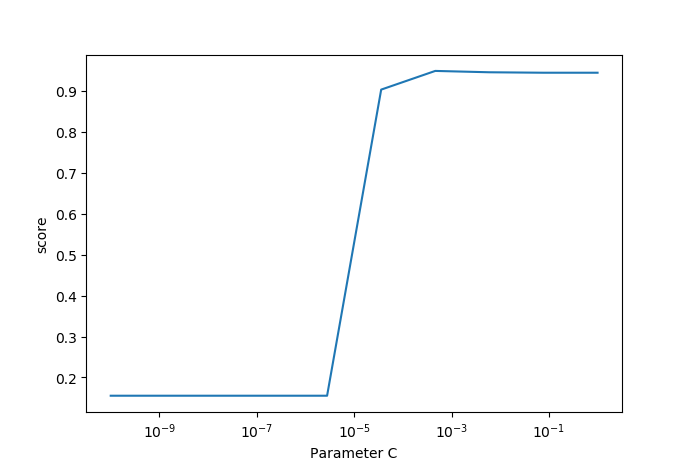
\includegraphics[scale=0.6]{ex904}
\end{slide}

\begin{slide}{Résultat attendu (2)}
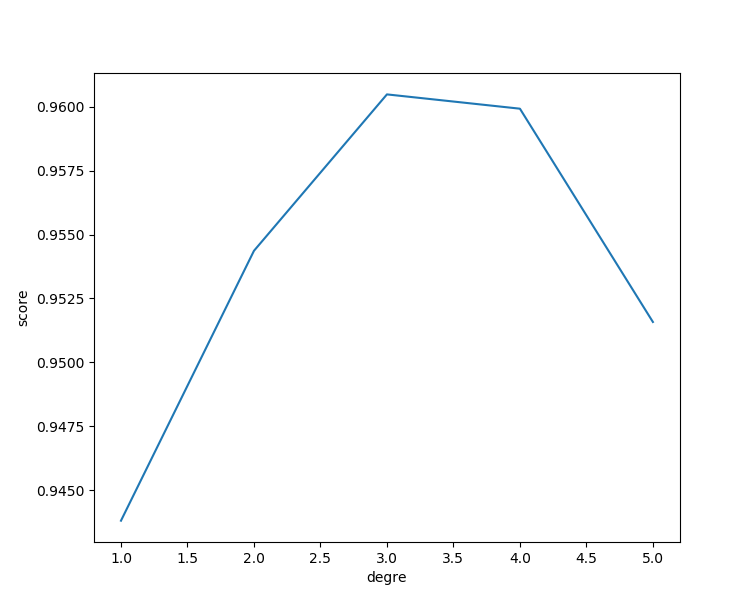
\includegraphics[scale=0.6]{ex905}
\end{slide}

\begin{slide}{solution}
\Python{ex904}
\end{slide}
\begin{slide}{solution}
\Python{ex905}
\end{slide}

\end{document}